
% -------------------------------------------
% Items to substitute into the ivoatex document template.
%
%\ivoagroup{Data Model Working Group}

%\title{Astronomical Coordinates and Coordinate Systems}


%\author{Arnold Rots}
    
%\author{Mark Cresitello-Dittmar}
    
%\author{Omar Laurino}
    
%\previousversion{0}
      
% -------------------------------------------

\pagebreak
\section{Model: coords }
  
  % INSERT FIGURE HERE
  \begin{figure}[h]
  \begin{center}
    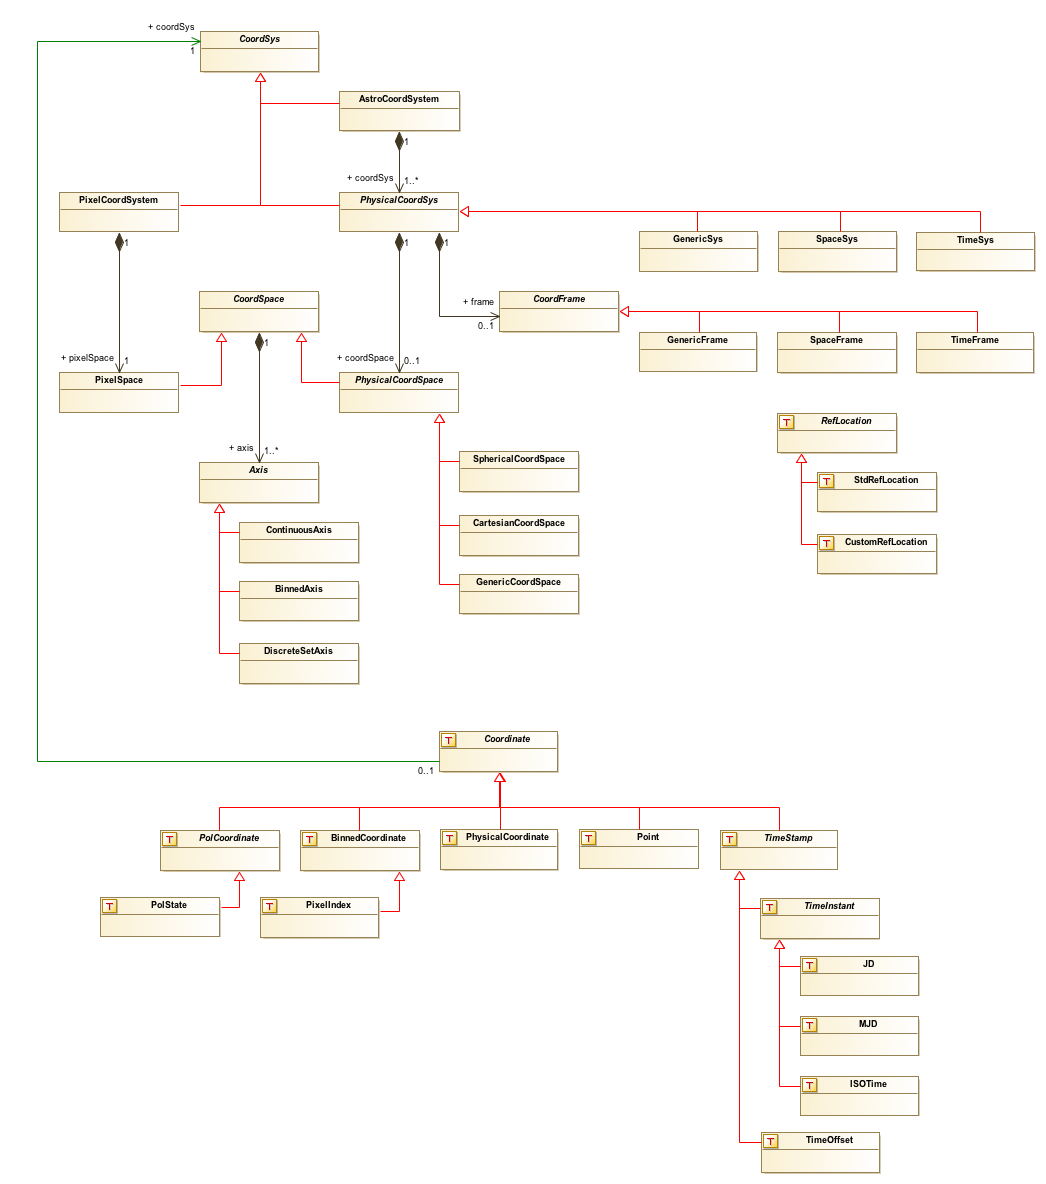
\includegraphics[width=\textwidth]{diagrams/Overview.png}
    \caption{Model Overview}\label{fig:overview}
  \end{center}
  \end{figure}

  This model defines objects which describe the coordinate space, coordinates within that space, and frames, which provide additional metadata regarding the origin, orientation, etc, of the coordinate space. The model also defines a coordinate system, bundling frames into associated groups.

\pagebreak
\section{Coordinates}

  % INSERT FIGURE HERE
  \begin{figure}[h]
  \begin{center}
    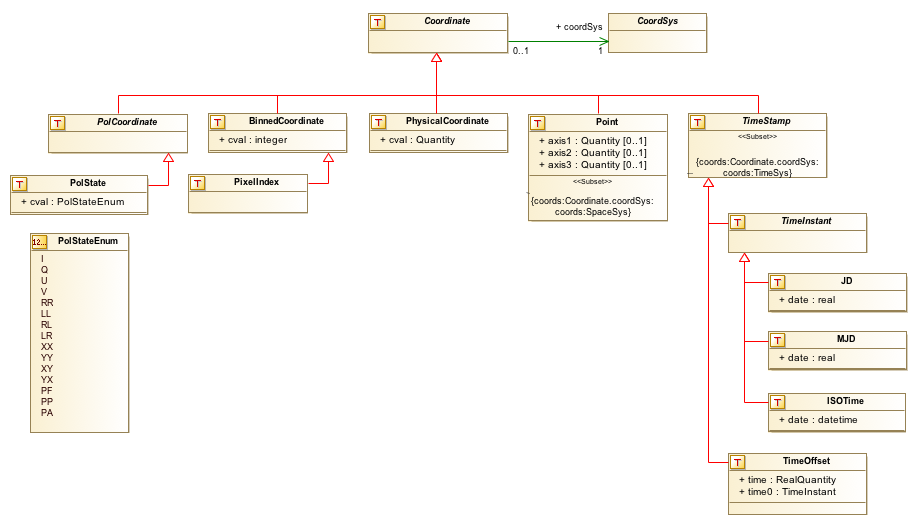
\includegraphics[width=6in]{diagrams/Coordinates.png}
    \caption{Coordinate elements}\label{fig:coordinates}
  \end{center}
  \end{figure}

  This section provides support for the most commonly used coordinate types.  The design allows for the specification of custom coordinate spaces, but leverages the fact that most data will reside in well defined standard spaces.  \textbf{It is expected that these coordinates will be used in the vast majority of cases.}


  \subsection{Coordinate (Abstract)}
  \label{sect:Coordinate}
    Abstract base class for the Coordinate data types which represent an absolute location within a coordinate space. Coordinates MUST refer to a coordinate system, providing additional metadata relevant to interpreting the coordinate value, and its representation.

    \subsubsection{Coordinate.coordSys}
      \textbf{vodml-id: Coordinate.coordSys} \newline
      \textbf{type: \hyperref[sect:CoordSys]{coords:CoordSys}} \newline
      \textbf{multiplicity: 1} \newline 
      Provided additional metadata relevant to interpreting the coordinate value; for example, the spatial reference position, or time scale, axis descriptions.


  \subsection{BinnedCoordinate}
  \label{sect:BinnedCoordinate}
    Coordinate value type specifically intended for binned data (e.g.: pixel indexes).

    \subsubsection{BinnedCoordinate.cval}
      \textbf{vodml-id: BinnedCoordinate.cval} \newline
      \textbf{type: \hyperref[sect:ivoa]{ivoa:integer}} \newline
      \textbf{multiplicity: 1} \newline 
      The binned coordinate value, expressed as an integer. e.g.: bin number, pixel index.


  \subsection{PhysicalCoordinate}
  \label{sect:PhysicalCoordinate}
    The most common type of coordinate value. This type is appropriate for any data whose values can be described by an ivoa:Quantity (numeric, with unit).

    \subsubsection{PhysicalCoordinate.cval}
      \textbf{vodml-id: PhysicalCoordinate.cval} \newline
      \textbf{type: \hyperref[sect:ivoa]{ivoa:Quantity}} \newline
      \textbf{multiplicity: 1} \newline 
      This coordinate MUST contain a value expressed as an ivoa:Quantity.


  \subsection{Point (Abstract)}
  \label{sect:Point}
    Multi-dimensional spatial coordinate. The Point MUST refer to a spatial coordinate system (SpaceSys) which associates the point with corresponding coordinate domain space and frame metadata.

    \noindent \textbf{subset} \newline
    \indent   \textbf{role: coords:Coordinate.coordSys} \newline
    \indent   \textbf{type: coords:SpaceSys} \newline


  \subsection{CartesianPoint}
  \label{sect:CartesianPoint}
    A spatial coordinate in a Cartesian coordinate space. Any associated CoordSpace MUST be a CartesianCoordSpace. If no CoordSpace is provided, a Standard Cartesian CoordSpace is assumed. Values for unused/undefined dimensions need not be provided.

    \subsubsection{CartesianPoint.x}
      \textbf{vodml-id: CartesianPoint.x} \newline
      \textbf{type: \hyperref[sect:ivoa]{ivoa:Quantity}} \newline
      \textbf{multiplicity: 0..1} \newline 
      The coordinate value along the 'X' axis.

    \subsubsection{CartesianPoint.y}
      \textbf{vodml-id: CartesianPoint.y} \newline
      \textbf{type: \hyperref[sect:ivoa]{ivoa:Quantity}} \newline
      \textbf{multiplicity: 0..1} \newline 
      The coordinate value along the 'Y' axis.

    \subsubsection{CartesianPoint.z}
      \textbf{vodml-id: CartesianPoint.z} \newline
      \textbf{type: \hyperref[sect:ivoa]{ivoa:Quantity}} \newline
      \textbf{multiplicity: 0..1} \newline 
      The coordinate value along the 'Z' axis.


  \subsection{LonLatPoint}
  \label{sect:LonLatPoint}
    A spatial coordinate in a Spherical coordinate space defining a Celestial position in Latitude and Longitude. Any associated CoordSpace MUST conform to this description. If no CoordSpace is provided, a Standard Spherical CoordSpace is assumed. Values for unused/undefined dimensions need not be provided.

    \subsubsection{LonLatPoint.lon}
      \textbf{vodml-id: LonLatPoint.lon} \newline
      \textbf{type: \hyperref[sect:ivoa]{ivoa:Quantity}} \newline
      \textbf{multiplicity: 0..1} \newline 
      The longitude of the Point, as a Quantity with angular units.

    \subsubsection{LonLatPoint.lat}
      \textbf{vodml-id: LonLatPoint.lat} \newline
      \textbf{type: \hyperref[sect:ivoa]{ivoa:Quantity}} \newline
      \textbf{multiplicity: 0..1} \newline 
      The latitude of the Point, as a Quantity with angular units.

    \subsubsection{LonLatPoint.dist}
      \textbf{vodml-id: LonLatPoint.dist} \newline
      \textbf{type: \hyperref[sect:ivoa]{ivoa:Quantity}} \newline
      \textbf{multiplicity: 0..1} \newline 
      The distance to the Point from the origin.


  \subsection{GenericPoint}
  \label{sect:GenericPoint}
    GenericPoint supports the representation of spatial coordinates in a custom coordinate space, or any space which is not covered by the other specializations. The coordinate values map, in order, to the axes described by the associated CoordSpace. If no CoordSpace is provided, the behavior is undefined. Values for unused/undefined dimensions need not be provided.

    \subsubsection{GenericPoint.axis1}
      \textbf{vodml-id: GenericPoint.axis1} \newline
      \textbf{type: \hyperref[sect:ivoa]{ivoa:Quantity}} \newline
      \textbf{multiplicity: 0..1} \newline 
      Coordinate value along the first axis of the associated coordinate space, expressed as an ivoa:Quantity.

    \subsubsection{GenericPoint.axis2}
      \textbf{vodml-id: GenericPoint.axis2} \newline
      \textbf{type: \hyperref[sect:ivoa]{ivoa:Quantity}} \newline
      \textbf{multiplicity: 0..1} \newline 
      Coordinate value along the second axis of the associated coordinate space, expressed as an ivoa:Quantity.

    \subsubsection{GenericPoint.axis3}
      \textbf{vodml-id: GenericPoint.axis3} \newline
      \textbf{type: \hyperref[sect:ivoa]{ivoa:Quantity}} \newline
      \textbf{multiplicity: 0..1} \newline 
      Coordinate value along the third axis of the associated coordinate space, expressed as an ivoa:Quantity.


  \subsection{TimeStamp (Abstract)}
  \label{sect:TimeStamp}
    This is the abstract basis for a set of simple time domain coordinates which are expected to accommodate the vast majority of use cases. All TimeStamps, by definition, exist in a standard 1-D coordinate space, with domainMin|Max of +/-Infinity. All TimeStamps MUST refer to an appropriate TimeSys.

    A Brief Primer on Time Metadata; for reference and more information, see: FITS WCS Paper IV \citep{2015A+A...574A..36R}.
    \begin{enumerate}
    \item  Required:\newline
     * Record time stamps in JD, MJD, ISO-8601, or elapsed time. If in elapsed time, a zero point MUST be given in a time stamp which is not itself an elapsed time. \newline
     * Provide the time scale used (e.g. TT, TDB, TAI, GPS, ET, UTC, TCG, TCB). \newline
     * Provide the reference position (place where the time is measured).
    \item  Note the following:  \newline
     * JD and MJD do not imply a time scale; it needs to be provided separately.  \newline
     * JD and MJD are dimensionless, though a unit of 'day' is implied.  \newline
     * It is a bad idea to mix UTC with JD or MJD, since not all UTC days are the same length. Instead, use the restricted form of ISO-8601: [[+|-]c]ccyy-mm-dd[Thh[:mm[:ss[.ss...]]]], with no time zone characters. \newline
     * TDB runs on average synchronously with TT, but corrects for the relativistic effects caused by deviations in the orbit of the Earth from perfect circularity and constant gravitational potential. \newline
    \item Recommendations:  \newline
     * Avoid UTC. It is trivial to convert the times provided by, e.g., space agencies, to TT immediately when you get them, and it will save headaches later on.  \newline
     * Use TT: it is the official IAU time scale, continuous with ET and the one which solar system ephemerides are based upon.  \newline
     * TAI and GPS are acceptable alternatives, with constant offsets from TT.  \newline
     * Use the same reference position for time and space and make sure it is commensurate with your time scale. For instance, when you convert to the barycenter, also convert to TDB.  \newline
     * Be aware that the barycenter is not the heliocenter  \newline
     * Be specific in labeling the time axis; e.g.: JD(TT;GEOCENTER) or MJD(TDB; BARYCENTER).  \newline
     * Use proleptic Gregorian dates for ISO-8601.
    \item Never use:  \newline
     * TJD, HJD, BJD, etc. These are not officially recognized and suggest certain metadata values, but leave considerable ambiguity as to what those metadata values actually are. Instead, specify your metadata explicitly. It avoids confusion later on and is not much more work.
    \item What if you deal with incomplete data?  \newline
     * If you do not know the time scale and/or reference position, you can provide them as UNKNOWN and set the systematic error/uncertainty to, say, 1000 s. 100 s will do if only the time scale is unknown.
    \item What else is there to know?  \newline
     * Quite a lot, especially the so-called coordinate time scales (TCG and TCB). Because TDB runs, on average, synchronously with TT, but in a very different potential well, which requires different values for fundamental physical constants in the barycenter. That is awkward and the coordinate time scales fix that by running at different rates. More in the above cited A\&A paper.\newline
    \end{enumerate}

    \noindent \textbf{subset} \newline
    \indent   \textbf{role: coords:Coordinate.coordSys} \newline
    \indent   \textbf{type: coords:TimeSys} \newline

  \subsection{TimeInstant (Abstract)}
  \label{sect:TimeInstant}
    TimeStamps which specify a specific instant in time. We define three subtypes (ISOTime, JD, MJD), which allow users to explicitly identify the representation and interpretation of the TimeInstant.

  \subsection{ISOTime}
  \label{sect:ISOTime}
    Extension of TimeInstant for time expressed as a structured datetime string. The string representation of a datetime value should follow the FITS convention for representing dates (Hanish and Farris et al, 2001). The FITS standard is effectively ISO8601 format without the 'Z' tag to indicate UTC: YYYY-MM-DD['T'hh:mm:ss[.SSS]]. The TimeScale is provided in the associated TimeFrame.

    \subsubsection{ISOTime.date}
      \textbf{vodml-id: ISOTime.date} \newline
      \textbf{type: \hyperref[sect:ivoa]{ivoa:datetime}} \newline
      \textbf{multiplicity: 1} \newline 
      The ISOTime coordinate value.

  \subsection{JD}
  \label{sect:JD}
    Extension of TimeInstant for time expressed in Julian days. Note that JD does not properly specify a time stamp unless it is related to a time scale and reference position. Precision can easily become an issue with JD, as the numbers tend to be large.

    \subsubsection{JD.date}
      \textbf{vodml-id: JD.date} \newline
      \textbf{type: \hyperref[sect:ivoa]{ivoa:real}} \newline
      \textbf{multiplicity: 1} \newline 
      The JD coordinate value. JD dates are dimensionless, with implied units in days.

  \subsection{MJD}
  \label{sect:MJD}
    Extension of TimeInstant for time expressed in Modified Julian Days. T(MJD) = T(JD) - 2400000.5.

    \subsubsection{MJD.date}
      \textbf{vodml-id: MJD.date} \newline
      \textbf{type: \hyperref[sect:ivoa]{ivoa:real}} \newline
      \textbf{multiplicity: 1} \newline 
      The MJD coordinate value. MJD dates are dimensionless, with implied units in days.

  \subsection{TimeOffset}
  \label{sect:TimeOffset}
    Time is given as an offset from a specific point in time (time0).

    \subsubsection{TimeOffset.time}
      \textbf{vodml-id: TimeOffset.time} \newline
      \textbf{type: \hyperref[sect:ivoa]{ivoa:RealQuantity}} \newline
      \textbf{multiplicity: 1} \newline 
      The TimeOffset coordinate value.

    \subsubsection{TimeOffset.time0}
      \textbf{vodml-id: TimeOffset.time0} \newline
      \textbf{type: \hyperref[sect:TimeInstant]{coords:TimeInstant}} \newline
      \textbf{multiplicity: 1} \newline 
      The reference time from which the offset is calculated. This MUST be given as a TimeInstant (e.g.: JD, MJD, ISOTime).


  \subsection{PixelIndex}
  \label{sect:PixelIndex}
    Specialized BinnedCoordinate for the pixel domain for a 1-dimensional pixel index. PixelIndex MUST refer to a PixelCoordSystem.


  \subsection{PolCoordinate (Abstract)}
  \label{sect:PolCoordinate}
    Abstract head of the polarization coordinate types. Current use cases only require support for discrete polarization states, however, we include this head class to facilitate extension for other types (eg: polarization fraction and angle).

  \subsection{PolState}
  \label{sect:PolState}
    Coordinate type for discrete polarization states.

    \subsubsection{PolState.cval}
      \textbf{vodml-id: PolState.cval} \newline
      \textbf{type: \hyperref[sect:PolStateEnum]{coords:PolStateEnum}} \newline
      \textbf{multiplicity: 1} \newline 
      The coordinate value MUST be from the PolStateEnum enumerated set.


  \subsection{PolStateEnum}
  \label{sect:PolStateEnum}

  Polarization states: Stokes, Circular, Linear and Vector states

  \noindent \underline{Enumeration Literals}
  \vspace{-\parsep}
  \small
  \begin{itemize}
  
    \item[\textbf{I}]: \textbf{vodml-id:} PolStateEnum.I 
    \item[\textbf{Q}]: \textbf{vodml-id:} PolStateEnum.Q 
    \item[\textbf{U}]: \textbf{vodml-id:} PolStateEnum.U 
    \item[\textbf{V}]: \textbf{vodml-id:} PolStateEnum.V 
    \item[\textbf{RR}]: \textbf{vodml-id:} PolStateEnum.RR 
    \item[\textbf{LL}]: \textbf{vodml-id:} PolStateEnum.LL 
    \item[\textbf{RL}]: \textbf{vodml-id:} PolStateEnum.RL 
    \item[\textbf{LR}]: \textbf{vodml-id:} PolStateEnum.LR 
    \item[\textbf{XX}]: \textbf{vodml-id:} PolStateEnum.XX 
    \item[\textbf{YY}]: \textbf{vodml-id:} PolStateEnum.YY 
    \item[\textbf{XY}]: \textbf{vodml-id:} PolStateEnum.XY 
    \item[\textbf{YX}]: \textbf{vodml-id:} PolStateEnum.YX 
    \item[\textbf{PF}]: \textbf{vodml-id:} PolStateEnum.PF 
    \item[\textbf{PP}]: \textbf{vodml-id:} PolStateEnum.PP 
    \item[\textbf{PA}]: \textbf{vodml-id:} PolStateEnum.PA 
  \end{itemize}
  \normalsize


\pagebreak
\section{Coordinate Frames}

  % INSERT FIGURE HERE
  \begin{figure}[h]
  \begin{center}
    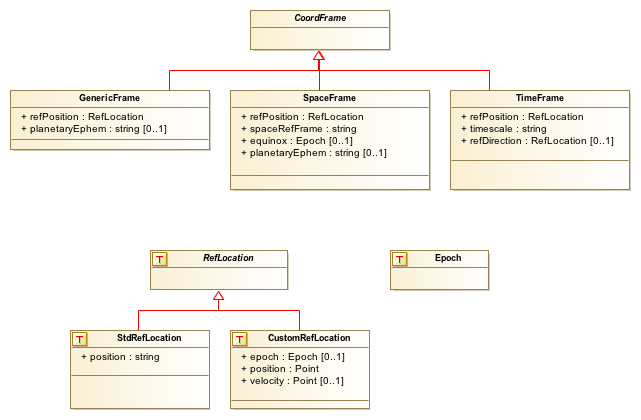
\includegraphics[width=4.5in]{diagrams/CoordFrame.png}
    \caption{Coordinate Frame elements}\label{fig:coordframe}
  \end{center}
  \end{figure}

  \subsection{CoordFrame (Abstract)}
  \label{sect:CoordFrame}
    This is the abstract, empty, base class for all coordinate frames. Coordinate frames provide metadata associated with the coordinate domain space. Typically, this will be related to the origin and orientation of the axes, but might include any metadata which pertains to the definition of the domain.

  \subsection{GenericFrame}
  \label{sect:GenericFrame}
    The generic coordinate frame is for cases where a domain-specific frame (e.g.: Space, Time), is not required, but the relevant reference metadata is still needed (e.g.: for Redshift or Spectral data)

    \subsubsection{GenericFrame.refPosition}
      \textbf{vodml-id: GenericFrame.refPosition} \newline
      \textbf{type: \hyperref[sect:RefLocation]{coords:RefLocation}} \newline
      \textbf{multiplicity: 1} \newline 
      Spatial location in phase space (position and velocity) at which the observed value is considered to have been taken. This will typically be given by a standard reference position, but we allow for custom locations as well.

    \subsubsection{GenericFrame.planetaryEphem}
      \textbf{vodml-id: GenericFrame.planetaryEphem} \newline
      \textbf{type: \hyperref[sect:ivoa]{ivoa:string}} \newline
      \textbf{multiplicity: 0..1} \newline 
      A planetary ephemeris MAY be provided, and SHOULD be provided whenever appropriate, to indicate which solar system ephemeris was used. If needed, but not provided, it is assumed to be "DE405"

  \subsection{SpaceFrame}
  \label{sect:SpaceFrame}
    A SpaceFrame is specified by its reference frame (orientation), and a reference position (origin). Currently only standard reference frames are allowed. An equinox MUST be provided for pre-ICRS reference frames. A planetary ephemeris MAY be provided if relevant. If needed, but not provided, it is assumed to be "DE405".

    \subsubsection{SpaceFrame.refPosition}
      \textbf{vodml-id: SpaceFrame.refPosition} \newline
      \textbf{type: \hyperref[sect:RefLocation]{coords:RefLocation}} \newline
      \textbf{multiplicity: 1} \newline 
      The spatial location at which the coordinates are considered to have been determined. This model supports locations provided as either a standard reference position (e.g. GEOCENTER), or a coordinate specifying a custom location (e.g. long, lat, height ).

    \subsubsection{SpaceFrame.spaceRefFrame}
      \textbf{vodml-id: SpaceFrame.spaceRefFrame} \newline
      \textbf{type: \hyperref[sect:ivoa]{ivoa:string}} \newline
      \textbf{vocabulary: http://www.ivoa.net/rdf/refframe} \newline
      \textbf{multiplicity: 1} \newline
      The spatial reference frame. Values MUST be selected from the controlled vocabulary at the given URL.

    \subsubsection{SpaceFrame.equinox}
      \textbf{vodml-id: SpaceFrame.equinox} \newline
      \textbf{type: \hyperref[sect:Epoch]{coords:Epoch}} \newline
      \textbf{multiplicity: 0..1} \newline 
      Reference date for the frame, required for pre-ICRS reference frames.

    \subsubsection{SpaceFrame.planetaryEphem}
      \textbf{vodml-id: SpaceFrame.planetaryEphem} \newline
      \textbf{type: \hyperref[sect:ivoa]{ivoa:string}} \newline
      \textbf{multiplicity: 0..1} \newline 
      Ephemeris file for solar system objects SHOULD be specified whenever relevant.


  \subsection{TimeFrame}
  \label{sect:TimeFrame}
    A TimeFrame SHALL include a time scale and reference position. It MAY also include a reference direction.

    \subsubsection{TimeFrame.refPosition}
      \textbf{vodml-id: TimeFrame.refPosition} \newline
      \textbf{type: \hyperref[sect:RefLocation]{coords:RefLocation}} \newline
      \textbf{multiplicity: 1} \newline 
      The spatial location at which the coordinate is considered to have been taken. This model supports locations provided as either a standard reference position (e.g. GEOCENTER), or a coordinate specifying a custom location (e.g. long, lat, height).

    \subsubsection{TimeFrame.timescale}
      \textbf{vodml-id: TimeFrame.timescale} \newline
      \textbf{type: \hyperref[sect:ivoa]{ivoa:string}} \newline
      \textbf{vocabulary: http://www.ivoa.net/rdf/timescale} \newline
      \textbf{multiplicity: 1} \newline
      The time scale sets the reference frame. The value MUST be selected from the controlled vocabulary at the given URL.

    \subsubsection{TimeFrame.refDirection}
      \textbf{vodml-id: TimeFrame.refDirection} \newline
      \textbf{type: \hyperref[sect:RefLocation]{coords:RefLocation}} \newline
      \textbf{multiplicity: 0..1} \newline 
      The reference direction is needed if the time stamps are transformed to a time frame with a different reference position. In those situations, the solar system ephemeris also comes into play. See: FITS WCS Paper IV for details, but in short: The reference direction, presumably the direction to the thing being observed, is used in conjunction with the reference position and planetary ephemeris to determine the correction applied for the path length change. To be fully useful, one also needs to know the location at which the observation was made ( i.e. the observatory location), which is not considered to be Frame metadata.


  \subsection{Epoch}
  \label{sect:Epoch}
  We define epoch as a primitive data type with the expected form "<type><year>" where type = "J" or "B" for Julian or Besselian respectively, and year is expressed as a decimal year. e.g.: "B1950", "J2000.0"


  \subsection{RefLocation (Abstract)}
  \label{sect:RefLocation}
    RefLocation defines the origin of the spatial coordinate space. This location is represented either by a standard reference position (for which the absolute location in phase space is known by definition), or a specified point in another Spatial frame. This object is used as the origin of the SpaceFrame here, but also to specify the Spatial Reference Position (refPosition) associated with other domain Frames. For example, in the Time domain, the Spatial Reference Position indicates that the 'time' values are the time that the 'event' occured at that location, which might be different from the detector location.


  \subsection{StdRefLocation}
  \label{sect:StdRefLocation}
    An absolute a-priori known location in phase space (position and velocity). Values are selected from the StdRefPosition vocabulary. Considering that the GEOCENTER is really the only place for which we know the absolute location at all times, all other locations require the specification of a planetary ephemeris. LSR[KD] are reserved for spectral and reshift frames. TOPOCENTER (location of the observer) is special in that it assumes that the observing location is available through other means (e.g. a geographic location or an orbit ephemeris). RELOCATABLE is available for simulations. UNKNOWN should only be used if absolutely necessary.

    \subsubsection{StdRefLocation.position}
      \textbf{vodml-id: StdRefLocation.position} \newline
      \textbf{type: \hyperref[sect:ivoa]{ivoa:string}} \newline
      \textbf{vocabulary: http://www.ivoa.net/rdf/refposition} \newline
      \textbf{multiplicity: 1} \newline
      Standard reference location. Values MUST be selected from the controlled vocabulary at the given URL.


  \subsection{CustomRefLocation}
  \label{sect:CustomRefLocation}
    A custom reference location in phase space (position and velocity). Position and velocity are given as coordinates with an associated SpaceFrame. An epoch MAY be provided to further refine the location.

    \subsubsection{CustomRefLocation.epoch}
      \textbf{vodml-id: CustomRefLocation.epoch} \newline
      \textbf{type: \hyperref[sect:Epoch]{coords:Epoch}} \newline
      \textbf{multiplicity: 0..1} \newline 
      Epoch for the reference location.

    \subsubsection{CustomRefLocation.position}
      \textbf{vodml-id: CustomRefLocation.position} \newline
      \textbf{type: \hyperref[sect:Point]{coords:Point}} \newline
      \textbf{multiplicity: 1} \newline 
      The spatial coordinates of the reference location.

    \subsubsection{CustomRefLocation.velocity}
      \textbf{vodml-id: CustomRefLocation.velocity} \newline
      \textbf{type: \hyperref[sect:Point]{coords:Point}} \newline
      \textbf{multiplicity: 0..1} \newline 
      The velocity of the reference location.


\pagebreak
\section{Coordinate Systems}

  % INSERT FIGURE HERE
  \begin{figure}[h]
  \begin{center}
    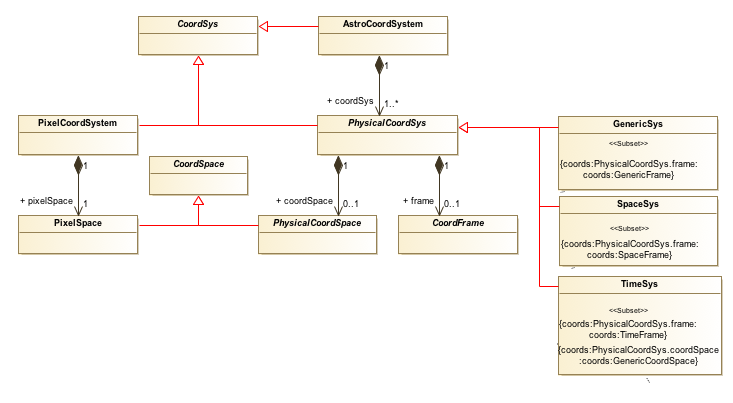
\includegraphics[width=5.25in]{diagrams/CoordSystems.png}
    \caption{Coordinate Systems }\label{fig:coordsys}
  \end{center}
  \end{figure}

  In the astronomical community, the term 'Coordinate System' is used to mean both ``the space in which a coordinate resides'', and ``a unique domain space'', folding in specific reference frame metadata.  In this model, we adopt the latter definition.  A Coordinate System provides a complete description of the domain space, including both the coordinate space description and associated Frame metadata.  To simplify the usage of these objects for the most common cases, we provide a set of standard CoordSpace instances which serve as defaults when not explicitely included in serializations.


  \subsection{CoordSys (Abstract)}
  \label{sect:CoordSys}
    Abstract head of the coordinate system object tree.


  \subsection{AstroCoordSystem}
  \label{sect:AstroCoordSystem}
    The AstroCoordSystem object holds a collection of component coordinate system descriptions across all represented physical domains.

    \subsubsection{AstroCoordSystem.coordSys}
      \textbf{vodml-id: AstroCoordSystem.coordSys} \newline
      \textbf{type: \hyperref[sect:PhysicalCoordSys]{coords:PhysicalCoordSys}} \newline
      \textbf{multiplicity: 1..*} \newline 
      Coordinate system description for each physical domain (Space, Time, etc).

  \subsection{PhysicalCoordSys (Abstract)}
  \label{sect:PhysicalCoordSys}
    Coordinate system description for any physical domain, such as Time, Space, Redshift, Temperature, Flux, etc.

    \subsubsection{PhysicalCoordSys.coordSpace}
      \textbf{vodml-id: PhysicalCoordSys.coordSpace} \newline
      \textbf{type: \hyperref[sect:PhysicalCoordSpace]{coords:PhysicalCoordSpace}} \newline
      \textbf{multiplicity: 0..1} \newline 
      Description of the coordinate space occupied by the property.

    \subsubsection{PhysicalCoordSys.frame}
      \textbf{vodml-id: PhysicalCoordSys.frame} \newline
      \textbf{type: \hyperref[sect:CoordFrame]{coords:CoordFrame}} \newline
      \textbf{multiplicity: 0..1} \newline 
      Associated Frame metadata.

  \subsection{PixelCoordSystem}
  \label{sect:PixelCoordSystem}
    The PixelCoordSystem provides a complete description of the pixel coordinate space. It SHALL contain one PixelSpace instance describing each pixel axis.

    \subsubsection{PixelCoordSystem.pixelSpace}
      \textbf{vodml-id: PixelCoordSystem.pixelSpace} \newline
      \textbf{type: \hyperref[sect:PixelSpace]{coords:PixelSpace}} \newline
      \textbf{multiplicity: 1} \newline 
      The pixel space completely defines the pixel coordinate axes.  Each axis MUST be defined as a BinnedAxis type.

  \subsection{GenericSys}
  \label{sect:GenericSys}
    Specialized coordinate system for generic, one-dimensional domains not covered by other, more concrete objects. If a CoordSpace is not provided, it is assumed to be represented by a Standard 1-Dimensional Coordinate Space as described in Appendix B.

    \noindent \textbf{subset} \newline
    \indent   \textbf{role: coords:PhysicalCoordSys.frame} \newline
    \indent   \textbf{type: coords:GenericFrame} \newline


  \subsection{SpaceSys}
  \label{sect:SpaceSys}
    Specialized coordinate system for the Spatial domain. This object SHOULD include an appropriate SpaceFrame. In Appendix B, we define two standard spatial coordinate space instances (Spherical and Cartesian), which may be referenced in serializations. If a CoordSpace is not provided, it is assumed to be represented by a Standard Spherical Coordinate Space.

    \noindent \textbf{subset} \newline
    \indent   \textbf{role: coords:PhysicalCoordSys.frame} \newline
    \indent   \textbf{type: coords:SpaceFrame} \newline


  \subsection{TimeSys}
  \label{sect:TimeSys}
    Specialized coordinate system for the Temporal domain. This object SHOULD include an appropriate TimeFrame. If a CoordSpace is not provided, it is assumed to be represented by a Standard 1-Dimensional Coordinate Space as described in Appendix B.

    \noindent \textbf{subset} \newline
    \indent   \textbf{role: coords:PhysicalCoordSys.frame} \newline
    \indent   \textbf{type: coords:TimeFrame} \newline


    \noindent \textbf{subset} \newline
    \indent   \textbf{role: coords:PhysicalCoordSys.coordSpace} \newline
    \indent   \textbf{type: coords:GenericCoordSpace} \newline


\pagebreak
\section{Coordinate Space}

  % INSERT FIGURE HERE
  \begin{figure}[h]
  \begin{center}
    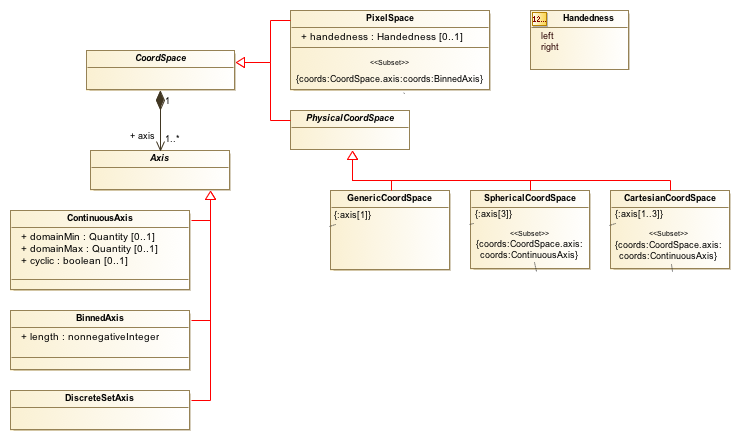
\includegraphics[width=5.25in]{diagrams/CoordSpace.png}
    \caption{Coordinate Spaces}\label{fig:coordspace}
  \end{center}
  \end{figure}

  \subsection{CoordSpace (Abstract)}
  \label{sect:CoordSpace}
    This object defines a domain space. i.e.: it describes the set of possible coordinate values.

    \subsubsection{CoordSpace.axis}
      \textbf{vodml-id: CoordSpace.axis} \newline
      \textbf{type: \hyperref[sect:Axis]{coords:Axis}} \newline
      \textbf{multiplicity: 1..*} \newline 
      Describes an axis of the coordinate space.


  \subsection{Axis (Abstract)}
  \label{sect:Axis}
    The abstract parent class for all coordinate axis types. We provide concrete classes for the most common types of data, Continuous, Binned, and Discrete, but allow extension for other types as needed.

    \subsubsection{Axis.name}
      \textbf{vodml-id: Axis.name} \newline
      \textbf{type: \hyperref[sect:ivoa]{ivoa:string}} \newline
      \textbf{multiplicity: 0..1} \newline 
      Freeform string, provides the name or label for the axis.

  \subsection{ContinuousAxis}
  \label{sect:ContinuousAxis}
    Axis description for continuous data. This object describes the domain for a particular axis of the domain space. It allows for the specification of the legal domain range (min,max), and a flag indicating if the axis is cyclic.

    \subsubsection{ContinuousAxis.domainMin}
      \textbf{vodml-id: ContinuousAxis.domainMin} \newline
      \textbf{type: \hyperref[sect:ivoa]{ivoa:Quantity}} \newline
      \textbf{multiplicity: 0..1} \newline 
      Minimum extent of the axis domain space. If not provided, the domain space is considered to have no lower bound (-INFINITY).

    \subsubsection{ContinuousAxis.domainMax}
      \textbf{vodml-id: ContinuousAxis.domainMax} \newline
      \textbf{type: \hyperref[sect:ivoa]{ivoa:Quantity}} \newline
      \textbf{multiplicity: 0..1} \newline 
      Maximum extent of the axis domain space. If not provided, the domain space is considered to have no upper bound (+INFINITY).

    \subsubsection{ContinuousAxis.cyclic}
      \textbf{vodml-id: ContinuousAxis.cyclic} \newline
      \textbf{type: \hyperref[sect:ivoa]{ivoa:boolean}} \newline
      \textbf{multiplicity: 0..1} \newline 
      Flag indicating if the axis is cyclic in nature. If not provided, it is assumed to be FALSE.

  \subsection{BinnedAxis}
  \label{sect:BinnedAxis}
    Axis description for binned data, where values along the axis correspond to a bin number.

    \subsubsection{BinnedAxis.length}
      \textbf{vodml-id: BinnedAxis.length} \newline
      \textbf{type: \hyperref[sect:ivoa]{ivoa:nonnegativeInteger}} \newline
      \textbf{multiplicity: 1} \newline 
      The length, or number of bins, along the axis.

  \subsection{DiscreteSetAxis}
  \label{sect:DiscreteSetAxis}
    Axis type specifically intended for enumerated coordinates. Since the content and nature of this axis type is heavily dependent on the use case, we define no additional metadata here. Extensions of this type may include additional metadata relevant to the particular use cases. For example, an extension could include the allowed set of values.


  \subsection{PhysicalCoordSpace (Abstract)}
  \label{sect:PhysicalCoordSpace}
    Abstract head of coordinate spaces related to physical properties.


  \subsection{SphericalCoordSpace}
  \label{sect:SphericalCoordSpace}
    Spatial domain, three-dimensional spherical coordinate space. The particulars of the axis descriptions depend on the flavor of space being instantiated. In Appendix B., we provide a Standard Spherical Coordinate Space instance which applies to many Astronomical use cases. It provides the default space for SpaceSys instances, and may be referenced in serializations.

    \noindent \textbf{subset} \newline
    \indent   \textbf{role: coords:CoordSpace.axis} \newline
    \indent   \textbf{type: coords:ContinuousAxis} \newline


    \noindent \textbf{constraint} \newline
    \indent    \textbf{detail: SphericalCoordSpace.axis[3] }\newline


  \subsection{CartesianCoordSpace}
  \label{sect:CartesianCoordSpace}
    Spatial domain, three-dimensional cartesian coordinate space. The particulars of the axis descriptions depend on the physical constraints of the instance. In Appendix B, we provide the description of a Standard Cartesian Coordinate Space instance which applies to many Astronomical cases, and may be referenced in serializations.

    \noindent \textbf{subset} \newline
    \indent   \textbf{role: coords:CoordSpace.axis} \newline
    \indent   \textbf{type: coords:ContinuousAxis} \newline


    \noindent \textbf{constraint} \newline
    \indent    \textbf{detail: CartesianCoordSpace.axis[1..3] }\newline


  \subsection{GenericCoordSpace}
  \label{sect:GenericCoordSpace}
    Generic, one-dimensional coordinate space suitable for use with most non-spatial properties. In Appendix B, we provide the description of a Standard 1D Coordinate Space instance which may be referenced in serializations.

    \noindent \textbf{constraint} \newline
    \indent    \textbf{detail: GenericCoordSpace.axis[1] }\newline


  \subsection{PixelSpace}
  \label{sect:PixelSpace}
  The Pixel coordinate space is defined as a 'virtual' binned space, with no physical meaning. The axes in this space provide integer indices into that space.  A PixelSpace SHALL include one or more BinnedAxis objects describing the pixel coordinate space. A handedness value MAY be provided to specify the relative orientation of the axes.

    \noindent \textbf{subset} \newline
    \indent   \textbf{role: coords:CoordSpace.axis} \newline
    \indent   \textbf{type: coords:BinnedAxis} \newline


    \subsubsection{PixelSpace.handedness}
      \textbf{vodml-id: PixelSpace.handedness} \newline
      \textbf{type: \hyperref[sect:Handedness]{coords:Handedness}} \newline
      \textbf{multiplicity: 0..1} \newline 
      Specifies the handedness of the coordinate space.


  \subsection{Handedness}
  \label{sect:Handedness}

  The handedness of a coordinate space. For most cases, this will be a fixed value in the specification of the coordinate space. We provide this element to allow this flexibility when needed. In this document, it is used in the Pixel domain.

  \noindent \underline{Enumeration Literals}
  \vspace{-\parsep}
  \small
  \begin{itemize}
  
    \item[\textbf{left}]: \textbf{vodml-id:} Handedness.left \newline
          \textbf{description:} positive x and y axes point right and up, the positive z axis points inward
    \item[\textbf{right}]: \textbf{vodml-id:} Handedness.right \newline
          \textbf{description:} positive x and y axes point right and up, the positive z axis points outward
  \end{itemize}
  \normalsize

